\section{Part 3 - Multivariable control}
\subsection{Problem 1}
Given the state variables:
\begin{equation}
  \boldsymbol{x} = \begin{bmatrix}
    \tilde{p} \\
    \dot{\tilde{p}} \\
    \dot{\tilde{e}} \\
  \end{bmatrix}
\end{equation}

and \cref{eq:linearized EoM}, the system matrices $\boldsymbol{A}$ and
$\boldsymbol{B}$ are as follows:

\begin{equation}
  \boldsymbol{A} = \begin{bmatrix}
    0 & 1 & 0 \\
    0 & 0 & 0 \\
    0 & 0 & 0 \\
  \end{bmatrix}, \hspace{0.5cm}
  \boldsymbol{B} = \begin{bmatrix}
    0 & 0 \\
    0 & K_1 \\
    K_2 & 0 \\
  \end{bmatrix}
\end{equation}

\subsection{Problem 2}
The rank of the controllability matrix, $\boldsymbol{\mathcal{C}}$, determines whether the system is controllable.


\begin{equation}
  \boldsymbol{\mathcal{C}} = \begin{bmatrix}
    \boldsymbol{B} & \boldsymbol{AB} & \boldsymbol{A^2B}
  \end{bmatrix}
  =
  \begin{bmatrix}
    0 & 0   & 0 & K_1 & 0 & 0\\
    0 & K_1 & 0 & 0   & 0 & 0\\
    K_2 & 0 & 0 & 0   & 0 & 0\\
  \end{bmatrix}
\end{equation}
which has full rank: $rank(\bm{\mathcal{C}}) = 3$, and is thus
controllable.

The system can be controlled by adding an LQR controller with reference
feed-forward, $u = \bm{Pr}-\bm{Kx}$. K is derived from the Matlab lqr
function, which requires the A and B matrices, in addition to
weighting matrices Q and R. When finding appropriate Q and R matrices,
Byrson's rule guided the first iteration. The rule states:

\begin{equation}
  Q_{ii} = \frac{1}{\text{maximum acceptable value of }x_i^2}
\end{equation}
\begin{equation}
  R_{jj} = \frac{1}{\text{maximum acceptable value of }u_j^2}
\end{equation}
where $x_i$ represents the $i^{th}$ state and $u_j$ represents the
$j^{th}$ input. All other entries to Q and R are 0. This resulted
in: \begin{equation}
  Q =
  \begin{bmatrix}
    1/(\pi/8)^2 & 0          & 0 \\
    0 &          1/(\pi/2)^2 & 0 \\
    0 &          0          & 1/(\pi/8)^2 \\
  \end{bmatrix}
  \qquad
  R =
  \begin{bmatrix}
    1 & 0 \\
    0 & 1 \\
  \end{bmatrix}
\end{equation}
These initial values represent the decision to have a small range of motion in
pitch, a large max speed in pitch to better control the pitch and a
relatively slow maximum speed in elevation. Furthermore, both inputs
max value is 1.

After tuning, the following Q and R matrices seemed to perform with
the quickest response without large overshoots:
\begin{equation}
  Q =
  \begin{bmatrix}
    60 & 0   & 0 \\
    0  & 0.01 & 0 \\
    0  & 0   & 100 \\
  \end{bmatrix}
  \qquad
  R =
  \begin{bmatrix}
    1 & 0 \\
    0 & 1 \\
  \end{bmatrix}
\end{equation}
A higher value for $q_{1,1}$ yields a more oscillatory pitch behavior,
while a lower value yields a slower response. As for $q_{2,2}$ a
higher value slowed the pitch response. With $q_{3,3} > 100$ the
system becomes difficult to control.
\todo[inline]{Explain why the system becomes difficult to control}

$\boldsymbol{P}$ is defined such that as time goes to infinity, the
states $\tilde{p}$ and $\dot{\tilde{e}}$ tend to their reference
values $\tilde{p}_c$ and $\dot{\tilde{e}}_c$. This happens when
$\dot{\boldsymbol{x}} = 0$, as the system reaches a stable equilibrium
around the reference values:

\begin{align*}
  \dot{\boldsymbol{x}} &= \boldsymbol{Ax} + \boldsymbol{Bu} \\
                       &= \boldsymbol{Ax} +
                         \boldsymbol{B}(\boldsymbol{Pr} -
                         \boldsymbol{Kx}) \\
                       &= (\boldsymbol{A}-\boldsymbol{BK})\boldsymbol{x}
                         + \boldsymbol{BPr} = 0
\end{align*}
When $\boldsymbol{\dot{x}} = 0$, $\boldsymbol{x}$ has reached its
final value, so $\boldsymbol{x} = \boldsymbol{x_\infty}$:

\begin{align*}
  (\boldsymbol{BK} - \boldsymbol{A})\boldsymbol{x_\infty} = \boldsymbol{BPr} \\
  \Leftrightarrow \boldsymbol{x_\infty} = (\boldsymbol{BK} - \boldsymbol{A})^{-1}\boldsymbol{BPr} \\
  \Rightarrow \boldsymbol{y_\infty} = \boldsymbol{Cx_\infty} = \boldsymbol{C}(\boldsymbol{BK} - \boldsymbol{A})^{-1}\boldsymbol{BPr}
\end{align*}
Therefore, the output $\boldsymbol{y_\infty}$ is equal to our reference $\boldsymbol{r}$ when:
\begin{equation}
  \boldsymbol{P} = [\boldsymbol{C}(\boldsymbol{BK} - \boldsymbol{A})^{-1}\boldsymbol{B}]^{-1}
\end{equation}
This achieves the desired result, that $\boldsymbol{y}$  goes to $\boldsymbol{r}$  as time goes to infinity:
\begin{align*}
  \lim_{t\to\infty}\boldsymbol{y}(t) = \boldsymbol{y_\infty} =
  \begin{bmatrix}
    \tilde{p} \\
    \dot{\tilde{e}}
  \end{bmatrix}
  =
  \begin{bmatrix}
    \tilde{p}_c \\
    \dot{\tilde{e}}_c
  \end{bmatrix}
  = \boldsymbol{r},
\end{align*}
\subsection{Problem 3}
With integral effect, the new state space matrices become:
\begin{equation}
  \boldsymbol{A} = \begin{bmatrix}
    0 & 1 & 0 & 0 & 0\\
    0 & 0 & 0 & 0 & 0\\
    0 & 0 & 0 & 0 & 0\\
    1 & 0 & 0 & 0 & 0\\
    0 & 0 & 1 & 0 & 0\\
  \end{bmatrix}, \hspace{0.5cm}
  \boldsymbol{B} = \begin{bmatrix}
    0 & 0 \\
    0 & K_1 \\
    K_2 & 0 \\
    0 & 0 \\
    0 & 0 \\
  \end{bmatrix}, \hspace{0.5cm}
  \boldsymbol{C} = \begin{bmatrix}
    1 & 0 & 0 & 0 & 0\\
    0 & 0 & 1 & 0 & 0\\
  \end{bmatrix}
\end{equation}

The matrices used to calculate the controllers gains, Q and R, also needed to be updated:

\begin{equation}
  Q =
  \begin{bmatrix}
    60 & 0   & 0  & 0 & 0 \\
    0  & 0.01 & 0  & 0 & 0 \\
    0  & 0   & 100 & 0 & 0 \\
    0  & 0   & 0  & 100 & 0 \\
    0  & 0   & 0  & 0 & 30 \\
  \end{bmatrix}
  \qquad
  R =
  \begin{bmatrix}
    1 & 0 \\
    0 & 1 \\
  \end{bmatrix}
\end{equation}

Without integral effect, the system could track pitch without much of
a problem. But the elevation rate had a noticeable deviation in the
ranges of elevation not close to our linearization point
$\dot{\tilde{e}} = 0$.

With integral effect, this deviation in elevation rate is
asymptotically removed. This means that with a zero Y output from our
joystick, there is a corresponding near zero elevation rate, and the
elevation angle also stays asymptotically constant for angles not
close to its linearization point.

Below, \cref{fig:Input_noIntegralEffect} and
\cref{fig:LQR_noEstimator} show the input and output of an automatic
run of the LQR controller without integral effect, while
\cref{fig:Input_IntegralEffect} and
\cref{fig:LQRIntegralEffect_noEstimator} show the input and output of
an automatic run of the LQR controller with integral effect. One
noticable difference in the input is the need for a small burst in y
at the beginning of the run to increase the helicopter to 0 degrees in
elevation. This is because this controller does a better job
regulating elevation rate, and with an input of 0, it would fly very
close to the table at the start. Aside from this the 2 input routines
are identical. The output is very similar in pitch and
travel. However, in elevation, at the end of the routine without
integral effect, the elevation angle returns to zero. While with
integral effect, although there is a bounce back, the controller does
not bring the helicopter's elevation angle back to zero, but instead
brings the elevation rate to zero.

\newgeometry{left=0.5cm,right=0.5cm,top=1cm,bottom=2cm}
\begin{figure}
  \caption{Input for no Integral Effect}
  \makebox[\textwidth][c]{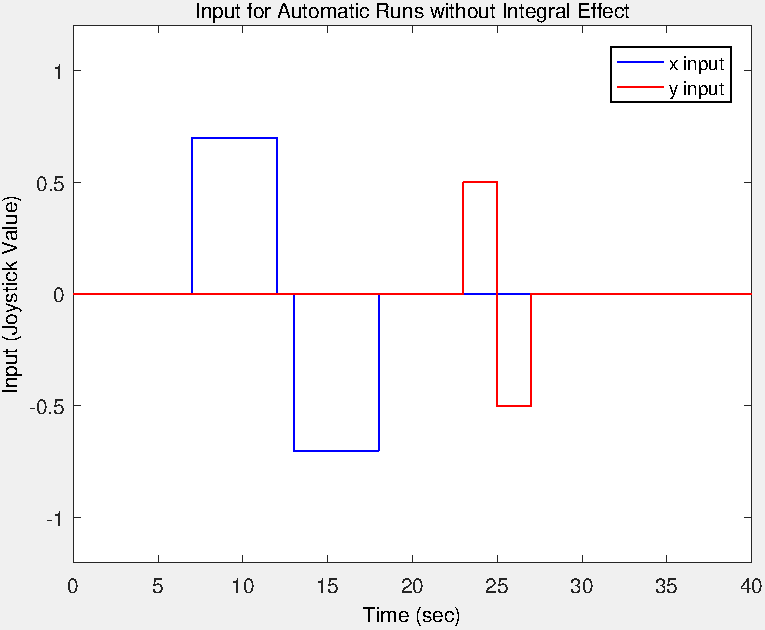
\includegraphics[height = 0.4\textheight]{images/input_noIntegralEffect.pdf}}
  \label{fig:Input_noIntegralEffect}
\end{figure}
%
\begin{figure}
  \caption{LQR Controller with no Integral Effect}
  \makebox[\textwidth][c]{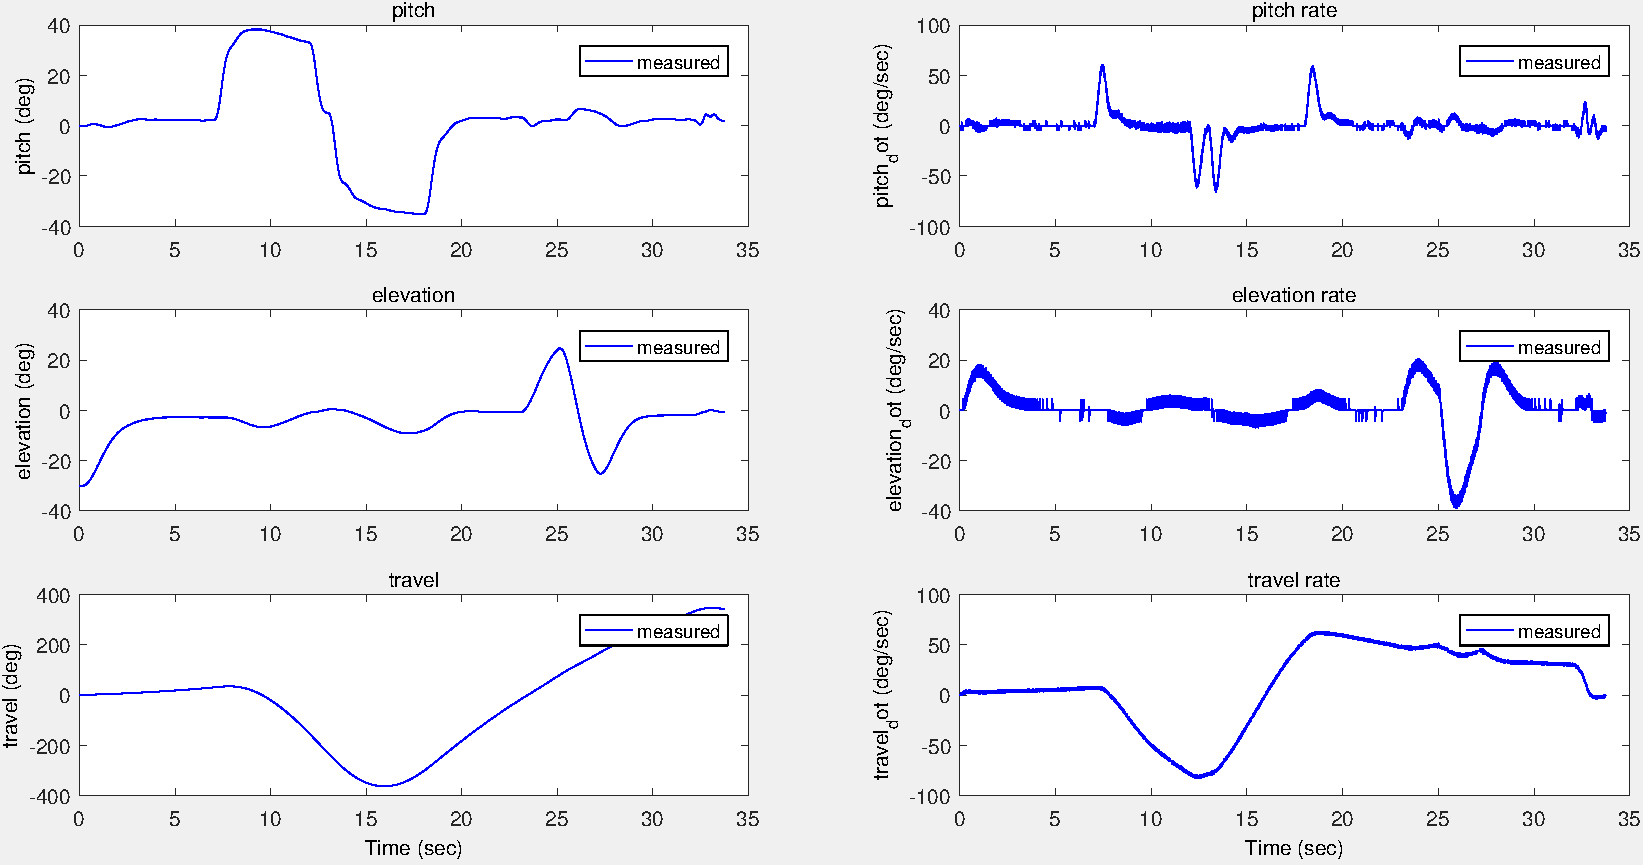
\includegraphics[width=\textwidth]{images/532_LQR_NoEstimator}}
  \label{fig:LQR_noEstimator}
\end{figure}
%
\begin{figure}
  \caption{Input with Integral Effect}
  \makebox[\textwidth][c]{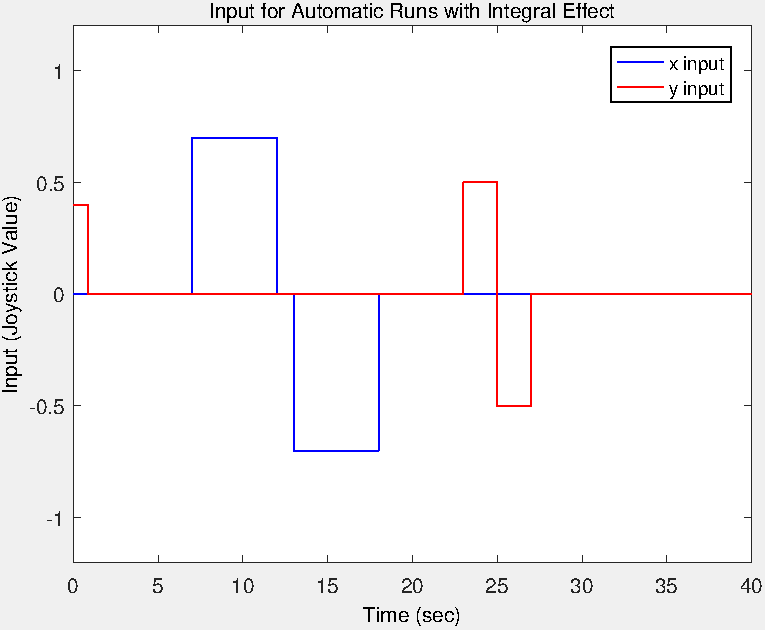
\includegraphics[height = 0.4\textheight]{images/input_IntegralEffect.pdf}}
  \label{fig:Input_IntegralEffect}
\end{figure}
%
\begin{figure}[hpb]
  \caption{LQR Controller with Integral Effect}
  \makebox[\textwidth][c]{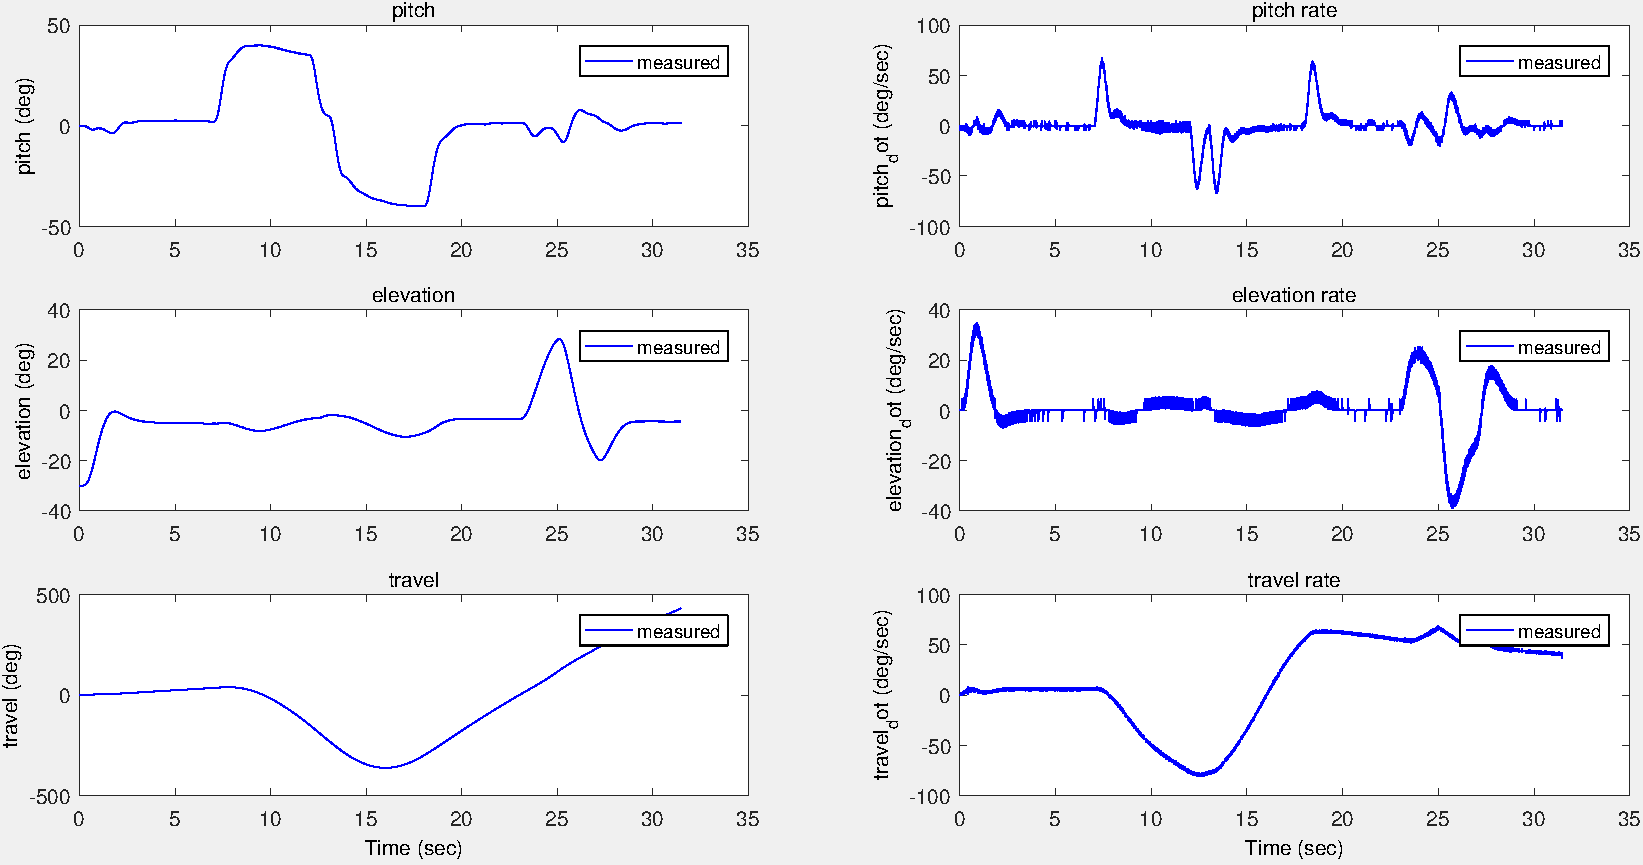
\includegraphics[width=\textwidth]{images/533_LQRIntegralEffect_NoEstimator}}
  \label{fig:LQRIntegralEffect_noEstimator}
\end{figure}
\restoregeometry

%%% Local Variables:
%%% mode: latex
%%% TeX-master: "report_main"
%%% End:
